\chapter{Model} \label{chapter:model}
  The model is the most important part of the project. An invalid model can only hope to produce an invalid simulation. This chapter will describe the model used during this project and compare it with the real world, noting and justifying any simplifications or assumptions used. The first section gives an overview of the model. The following sections then looks at specific parts in more detail.
  
  \section{Overview}
    The aim of modelling is to highlight which features in the environment to be simulated are important and which can be ignored\cite{Sterling2009}. For an agent-based model we wish to break these features down into the agents and their environment and their interactions with that environment so that the agents may assess their situation and make decisions\cite{Bonabeau2002}. In this section there is a summary of the important features of the model and their relationships.
    
    The agents in this model are coxes. The main features of their environment are the boat in which they sit, the boats containing other coxes and the river on which these boats sit. The coxes interact with the environment through actions which will determine how the boat behaves. The cox aiming to safely navigate the boat from one end of the river to the other. It should also be noted that at one end of the river sits a Boat House from which new boats are launched and to which a cox must return its boat and land.
    
    The model is cox-centric. For instance, the model does not aim to replicate how the rowers in a boat implement a cox's orders. However, the best way to describe the model is to work from the bottom up spatially.
    
    At the bottom is the river. This is the entity shared by all boats and defines the positional constraints placed upon them. Every boat must be fully on the river. The river is made up of 3 lanes which can be thought of as 1 dimensional spaces broken up by regular marker nodes, in other words a graph where each node represents a particular point on the river and each edge represents a connection to the next point in the lane either upstream or downstream (so each node only has one edge in and one edge out, though see the exception for changing lanes in \ref{model:river:lane_changing}). By mapping each node's location to a 2 dimensional space and assuming that there is a channel of water about 10 metres wide between each connected node, the river can then be drawn as the union of these lanes.
    
    In the middle is the boat. The boat can be considered as the embodiment of the cox. It is the boats that floats on the river and should not be allowed to overlap with the bank or another boat. When the cox carries out an action it is by altering properties of the boat such as it's speed and direction. No attempt has been made to model directly the rowers who in reality do the hard work of actually propelling the boat along the river. At each tick of the clock the boat will move, based on the current value of its properties, which may have just been altered by the cox. It should be noted that outside forces other than the cox can act on the boat. For instance, should two boats try and travel along the same edge in a lane then they will crash and come to a complete standstill for a while.
    
    At the top the cox sits in the boat. The cox can make observations about the state of its own boat and the river nearby (should the boat be travelling faster? are there any nearby boats? is the boat nearing the end of river?). At each tick of the clock the cox uses these observations to decide which action to perform next and then executes it. The actions themselves may show different behaviour depending on the boat's situation. For example, a boat at its maximum speed will not change speed even if the cox decides to execute the Speed Up action.
    
    One feature that sits slightly apart from the cox-boat-river layered view of the model is the Boathouse. It might itself be considered an agent since it launches boats, but as neither launching nor landing can be considered intelligent processes from the Boat House's point of view for the purposes of describing the model it fits more naturally as part of a part of the river since it also marks one end of the river beyond which a boat cannot pass.
    
    For the simulation, time is turned into discrete ticks. Methods are scheduled to run at ticks. For a cox, the \texttt{step()} method is scheduled to run every tick and carries out a full observe-decide-execute cycle, observing the state of the river and other boats on it, deciding what action to do next and then executing that action. For a boat the \texttt{run()} method will move the boat according to it's properties after the cox has executed their action (the scheduled method on coxes is given a higher priority so will run before the scheduled method on boats). At some ticks the Boat House will have a method scheduled to launch a boat.
    
    Figure \ref{fig:modeloverview} provides a summary the relations between the 4 main features of the model just described. The following sections describe in more detail the river, the boats and the coxes and their decision making processes.
    
    \begin{figure}
    \begin{center}
    	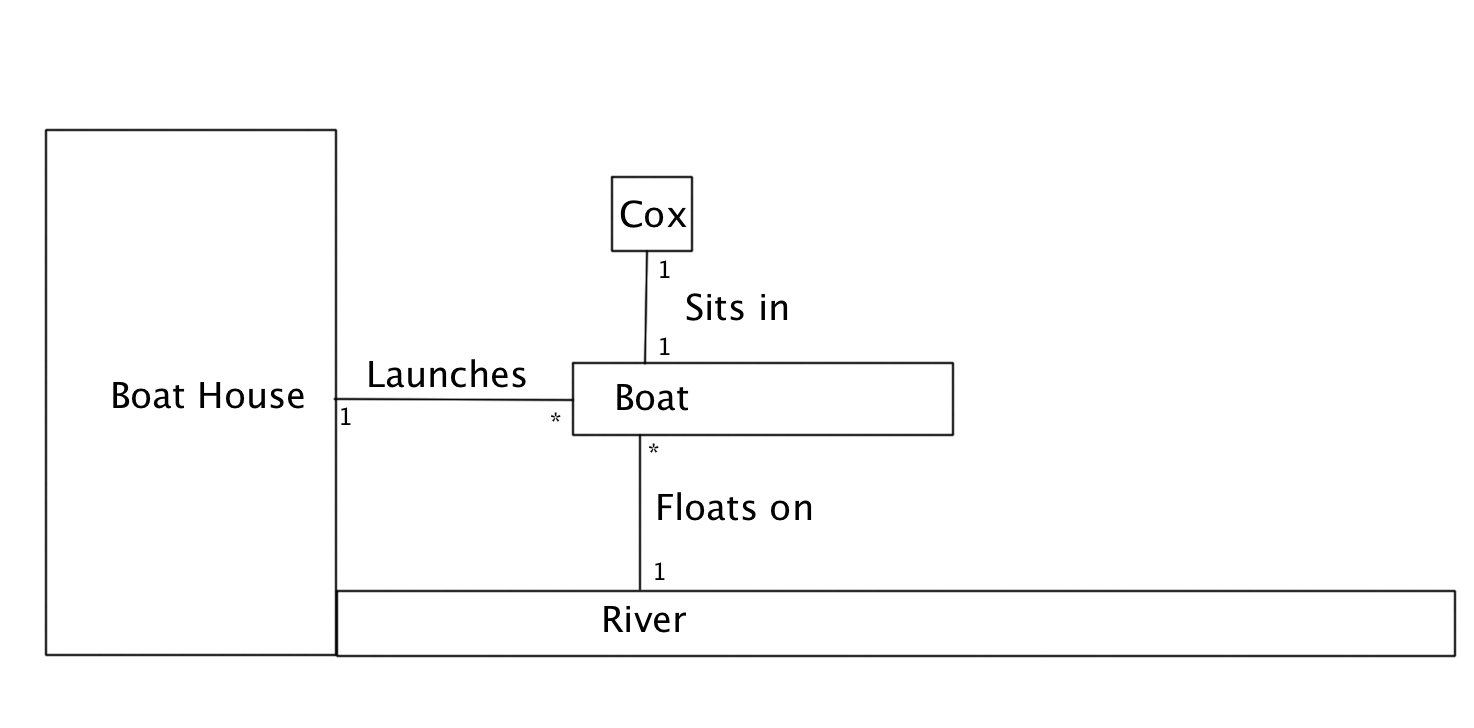
\includegraphics[scale=0.3]{images/ModelOverview.png}
    	\caption{Model Overview}
    	\label{fig:modeloverview}
    \end{center}
    \end{figure}

    \section{River}
      \subsection{Real world description}
      Most rowing on the Cam takes places in the 5km between Jesus Lock and Baits Bite Lock. A few crews sometimes carry their boats over Baits Bite Lock to another stretch of river up to Bottisham lock. The boathouses used by rowers are clustered near Jesus Lock. The first 2km from Jesus Lock are quite narrow and windy. This section is used for warm-ups and warm-downs and in theory on this part of the river crews are not supposed to row at full pressure. It is in the 3km up to Baits Bite lock that the most varied rowing takes place. The river has been known to flood but for the most part it is static and its stream has no effect on boats. The river bank is varied and there are many landmarks such as corners, bridges, trees, and buildings by the river. The width of the river varies between wide enough to allow 3 crews to be side-by-side down to a bottleneck where only one crew can pass at a time.
      
      \subsection{Simplified Model}
      
      \subsubsection{Lock}
      A crew carrying their boat over Baits Bite Lock happens infrequently enough that it can safely be ignored and Baits Bite Lock can be treated as the end of the river. Therefore the river can be considered to stop at Baits Bite lock. Other than acting as a barrier the lock has no other effect on boats and so no more work has gone into it. Indeed it is not even visualized in the simulation (the river just finishes).
      
      \subsubsection{Boathouse}
      The boathouses are all placed on the first 2km of the river from Jesus Lock and behaviour in this stretch of the river is sufficiently different that it is reasonable to merge this section of the river into a boathouse which marks the start of the river and only consider the final 3m of the river up to Baits Bite lock. It is from this Boathouse that boats are launched and to where boats aim to return at the end of their outing.
      
      A true traffic simulation modelling conditions on the Cam might aim to carefully replicate the launch rates, matching how they vary throughout the day, week and year, and types of boat launched (e.g. fast, experienced eights or slow, novice single sculls). However, this is beyond the scope of this project and unfortunately collecting this data is difficult as the traffic pattern changes drastically when the academic year ends in June. Instead the Boathouse will launch boats by following schedules generated randomly. This will still allow coxes to experience different situations such as busy periods lots of boats launching or quiet times with only a few boats out and generating schedules which match real world conditions more closely during follow-up work is not ruled out.
      
      \subsubsection{Simplification from 3D space to into three 1D lanes}
      The biggest simplification is to consider the river as three parallel lanes. Since the length of a boat is about the same as the width of the river it is safe to consider the lanes as 1D spaces along which the boat can move since it is only feasible for a boat to travel up and down the river (i.e. with or against the stream) but not feasible for a boat to travel to across the river other than briefly when changing lanes or spinning. The restriction to one dimension then makes it much simpler to move the boats around and detect collisions.
      
      Less justifiable is to have three lanes for the entire length of the Cam. For most of the river two-way traffic is possible but three-abreast traffic is limited to quite a small part. However, three lanes allow for some interesting behaviour with a central lane for overtaking. It also allows the assumption at any point on the river there is part of each of the three lanes nearby. Section \ref{model:river:lane_changing} on changing lanes could also be used a starting point for merging lanes. Unfortunately for this project the assumption of three lanes for the length of the river is deeply embedded so further work would be needed to remove it.
      
      While this project takes rowing on the Cam for inspiration as much as possible the software produced is able to simulate other three-laned rivers without much alteration. Details on how the lanes were created to match the Cam can be found in \ref{techissues:river}.
      
      \subsubsection{Lanes}\label{model:river:lanes}
      Each lane can be thought of as a simple directed graph with each node connected by one edge in and one edge out. By making the graph directed there is a unique node that is the next node depending on whether the boat is travelling downstream (away from the boathouse) or upstream (towards the boathouse) which map to travelling with the direction of the edges or against the direction of the edges. See Figure \ref{fig:model:lanes} for a diagram representing the 3 main lanes.
      
      \begin{figure}
      \begin{center}
      	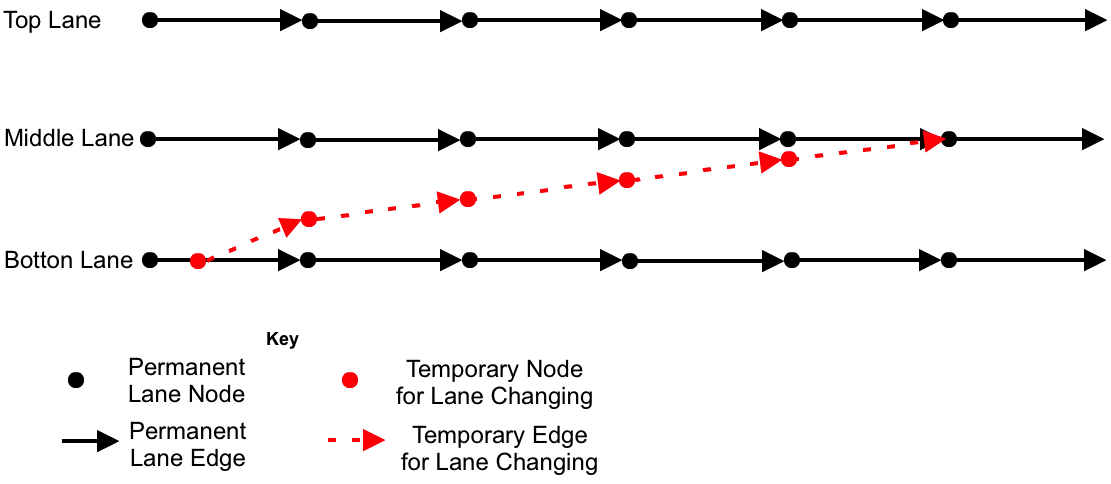
\includegraphics[scale=0.3]{images/lanes.png}
      	\caption{Representation of river as 3 lanes with a temporary path for lane changing}
      	\label{fig:model:lanes}
      \end{center}
      \end{figure}
      
      The nodes have a position attribute. They are a way of modelling the various landmarks scattered along the river which coxes can use to work out where they are.
      
      Each node is placed so its location is 20m from the next one in the graph. Therefore edges between the nodes have a length that is roughly the same as the length of a boat. This means a boat is considered to fill the edge as it travels between the nodes at either end. A boat will remain on an edge for as long as it takes to travel edge's length. Once the boat has covered this distance it will exit the current edge and occupy the next edge in the graph. This allows for a simple collision detection mechanism. If two or more boats try to occupy the same edge then they are considered to have crashed. More detail on crashing can be found in \ref{model:movement:crashing}.
      
      \subsubsection{Lane Changing} \label{model:river:lane_changing}
      The one edge in, one edge out rule is temporarily broken when a cox decides to change lane. In this case a new set of nodes and edges are temporarily added to the graph of the target node. These nodes and edges are marked so that other coxes will ignore them. These new nodes and edges start from the boat's current location and join up with a node further along in the target lane. These new nodes are located so that the cox will smoothly steer the boat into the new lane in the visualization. For collision detection purposes the boat is considered to occupy edges in both the starting lane and the target lane until the boat is fully in the the target lane and back to following the predefined graph of the target lane. When a boat is travelling along one of the red temporary edges in Figure \ref{fig:model:lanes}, it is considered to also occupy the two black permanent lanes sandwiching temporary edge above and below.

    \section{Boat}
      \subsection{Real world description}
      The river is used by rowing boats of various sizes both coxed and coxless. The river is also used by a few barges and riverboats. Many of these are lived in and never move from their moorings on the bank by the boathouses. A few do occasionally move up and down the river. The vast majority of these boats are well handled. The tourist traffic which behaves more erratically is restricted to a different part of the river. However, during term time the majority of river users are college crews and the nature of college racing means that the vast majority of rowing is done in eights, which are always coxed.
      
      A commonly used boat is a Janousek eight which is roughly 17m long, 60cm wide and 40cm deep (\cite{Janousek}). The effective width of an eight is much wider since the oars must be taken into account. An oar on a rowing boat is roughly 370cm long (\cite{Concept2}), although about 60cm of that will overlap with the boat itself. Therefore the effective width of an eight is more like 7m. The rowers can draw in their oars most of the way to reduce the width of the boat, but this should only be done on one side and when the boat is stationary if the rowers do not wish to capsize. 
      
      The rowers sit in the boat. The cox will control the amount of power applied by each rower as a proportion of each rower's maximum power. In this way indirectly set the speed of the boat. The maximum power of each rower is determined by his strength and skill which may be affected by factors such as fatigue. Not all boats are equal. Male rowers can apply more power than female rowers. Crews for a boats are selected by ability as well as gender so a 1st women's boat will be able to move faster than a men's 4th boat.
      
      Without orders to the contrary from the cox, a boat will continue to move forward at a constant speed. In part this is due to physics (even an eight a small women weighs over half a tonne). However, this is mainly due to the way rowers behave. Rowers are taught to carry on rowing unless the cox tells them to stop rather than being told to take each stroke individually.
      
      \subsection{Model Overview}\label{model:boat:simplified}
      For modelling purposes the boat is the object that is bound by the physical constraints of filling space around a particular location which should be entirely on the river. It is also the object moves according to its speed and orientation rather than the cox due to the indirect nature of a cox's control and the way that rowers are taught to behave. Therefore movement is a feature of the boat rather than the cox. Although the way in which the boat moves is determined by the cox's actions.
      
      \subsection{Space filling}
      As the most boats on the river are rowing eights it is reasonable to assume for our model all boats are rowing eights and for visualization purposes a boat fills a rigid 17m x 7m rectangle (though something that looks a little more like an eight is displayed, see Figure \ref{fig:model:boat}). More importantly for the model, since boats are restricted to lanes and each edge at 20m long is roughly the length of a boat, a boat fills an edge completely while it travels along it. This means that sometimes the visualization occasionally shows boats overlapping but not crashed. This is acceptable since the reality of the situation is there is some flexibility with drawing in oars and boats not filling a rectangle that can allow boats to travel very close together. Similarly, boats may appear not to be overlapping but still to have crashed. This also represents reality where coxes and coaches may get nervous and stop boats which get very close. Although using edge occupancy as a means of collision detection is rather crude for the scope of this project it is an acceptable simplification. A more accurate model would need to be a lot more complicated and would probably not provide much more accuracy to the simulation.
      
      \begin{figure}
      \begin{center}
      	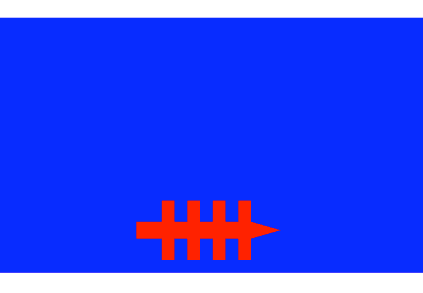
\includegraphics[scale=0.3]{images/boat.png}
      	\caption{What a boat looks like in the visualization. Boat is travelling left to right (so stern to the left, bow to the right).}
      	\label{fig:model:boat}
      \end{center}
      \end{figure}
      
      \subsection{Movement}
      As well as modelling how the boat physically fills space on the river, the boat is also the object that moves. During each tick after the cox has executed its action, the boat will follow the lane it is in at whatever speed it has (both of which may have been changed by the cox).
      
      \subsubsection{Speed}
      The speed of the boat is determined by which of 10 gears it is currently in and a speed multiplier. The gear represents the discrete ways a cox can alter the boat speed by altering the number of rowers active, the amount of power being applied by the rowers and the number strokes per minute taken by the rowers. The speed multiplier represents how ``good" the crew is. The boat's speed is the product of the gear and multiplier. Boats speed up and slow down instantly when instructed to do so by the cox. However, outside of crashing which will bring them to a stop, they will only be able to shift up or shift down a single gear at a time in order to mimic slightly the time it takes to accelerate a boat.
      
      No attempt has been made to model the rowers getting tired. The speed multiplier remains constant throughout an outing. Nor has any attempt been made to simulate the rowers misinterpreting the cox's instructions. Instead the boat will respond instantly and perfectly to the cox's instructions. This simplification was necessary due to the time restrictions of the project. It is certainly part of the model that should be looked at in more detail in the future since one of the interesting aspects of the cox-boat relationship is the indirect control that cox has over the boat and the time it takes from a cox deciding to carry out an action, giving the crew an order and then the crew carrying out the order.
      
      \subsubsection{Steering}
      As described in \ref{model:river:lanes}, the river is broken down into nodes that to represent landmarks corresponding to a position on the river. This means they can be used to model a cox's vision. A cox knows at certain position he needs to so they know how to steer safely along the river. When the boat reaches a node in the lane it will automatically adjust its orientation to point towards the next node. Effectively the cox automatically steers around the river and so for simplicity it has been absorbed into boat movement. This allows the simulation to focus on the interactions between the coxes rather than the cox having to learn how to avoid the bank, which is unchanging and hitting the river bank would never be a sensible course of action. It is not an unreasonable simplification for an experienced cox who will find that steering the river course becomes automatic anyway and it is only when avoiding moving obstacles like other boats that a cox will knowingly think about steering. More on this part of steering can be found in the Changing Lane action in \ref{model:cox:actions}.
      
      \subsection{Crashing}\label{model:movement:crashing}
      As well as modelling how the boat moves, it is also necessary to model when movement is not possible. That is when a boat crashes. Since steering to avoid the bank happens automatically, the crashes of interest are between multiple boats. For this project crashes are considered to cause delays when two or more boats get two close to each other. In theory a crash could be so bad that the boats are written off and the crew must get out and walk back. This is exceedingly rare. Therefore it is assumed that crashes are not catastrophic. Instead when boats get too close someone either in the boat or on the bank will shout at them all to stop. The crews will then take some time to put some space between each other. This may involve pushing each other away physically or one boat drawing its oars in so that another may pass, or a boat may chose to ``back it down", where the rowers will row backwards causing the boat to move slowly backwards.
        
      \subsubsection{Defining in model context}
      For the model boats are said to have crashed if they try and occupy the same permanent edge in one of the lanes that makes up the river. This is because a boat is considered to fill an edge entirely and therefore it does not make sense to have more than one boat travelling on the same edge.

      \subsubsection{Effects}
      When a boat tries to occupy an edge that already contains another boat then all the boats on the edge will be brought to a stop and the coxes will be rendered incapacitated for a fixed number of ticks. After this (assuming another boat does try and occupy the edge, which will cause the counter to reset), one of the boats will be picked at random and be allowed to move. When this boat gets clear of the edge, another boat will be selected at random and be allowed to move. And so on until all the boats have cleared the edge.
      
      The period where the coxes are incapacitated represents the time when boats must get clear of each other so they can begin rowing again. By keeping the boats stationary the delay caused by the crash is kept in the model without having to add the ability for backward movement to the boats. This means boats all move forward monotonically (with spinning changing the definition of what counts as forward) which makes reasoning with the model much simpler.
      
      A single boat is chosen because in most crashes there is a boat that can get clear first and the others will wait. A more accurate model might try and have a better guess than random at which boat this would be (for example if a boat rams the boat in front, it will be the boat in front that moves first) but a random selection is simpler to implement without much loss of accuracy.
      
      By allowing only one boat to move then it reduces the potential for boats to remain in a permanently crashed state as they boat crawl along impeded by each other. With only one boat chosen at random to move, eventually the faster boat will get clear.
      
    \section{Cox}
      \subsection{Description}
      \paragraph{Description of duties and abilities}
      The best way to describe a cox is to consider his duties and abilities. In all rowing boats, coxed or not, someone must carry out these duties and is given these abilities. The difference in a coxed boat is that there is an individual whose sole purpose and to carry out these duties with all the abilities. But the following still applies in non-coxed boats where the cox is an abstract quantity with the duties and abilities distributed amongst the crew.
      
      The cox controls the rudder with which the direction of the boat can be altered. The cox is the authority in the boat and all the rowers are supposed to carry out his commands. In particular the cox dictates the power applied by each rower which in turn dictates the boat speed. Therefore the cox is responsible for navigating the boat safely along the river, avoiding static obstacles like the bank and moving obstacles like other rowing boats. While the rowers are supposed to focus on their rowing, the cox is free to look around him in order to avoid these obstacles. 
      
      The cox is also responsible for carrying out the outing plan supplied by a coach, which specifies how fast the boat should be moving during various parts of the outing and how much distance the boat should cover during the outing. After all, travelling a short distance at a slow speed may reduce the risk of crashes but it will not help the boat to race quickly.
      
      To avoid distractions rowers are not supposed to talk while rowing. One of the cox's most important tools is his voice. Therefore the cox is supposed to coach and motivate the crew.
      
      \subsection{Cox Model Overview}
      As stated before the coxes are the autonomous agents in the model. Their actions (performed by the rowers or the rudder) affect the boat and determine in which direction and how fast the boat will move when it comes to calling the run() method on the boat object. For the most part this project will stick to having autonomous coxes deal the physical issues of guiding the boat. Although coaching and motivation are an important part of a real-world cox's duties, for the model the rowers shall be considered to respond perfectly to a cox's commands so that a cox's actions can be considered to have a direct effect on the boat.
      
      The layered agent-modelling technique laid out by Sterling and Taveter \cite{Sterling2009} is loosely followed to produce the cox model. First the goals the cox wishes to achieve and the constraints placed upon the cox are defined, then the actions available to the cox and the observations and knowledge base the cox can call on. Finally the observations and knowledge are used by the cox to decide which action is performed and when in order to achieve its goal bearing in mind the constraints placed upon it and the boat.

      \subsection{Goals \& Constraints}
      The overall goal for the cox is to make it back to the boathouse at the end of the outing. It is absolutely no good to leave a boat stranded in the middle of the river. Ideally the cox should be safe, so avoid hitting the river bank or colliding with other crews. If a collision is unavoidable, the relative speed of the collision should be as low as possible. The cox should also aim to maintain a speed as close as possible to outing speed and cover a distance as close as possible to the outing plan.
      
      The cox is not completely free to achieve the goals in any possible way. There are the physically that have been mentioned before. A boat must sit fully on the river and it cannot overlap with another boat. There are also rules for river use laid down by a governing body called CUCBC \cite{CUCBC}. Unlike the previous two hard, physical constraints these rules of the river (like rowing on the right-hand side) can be ignored. It would be interesting to see which of these rules get learnt naturally and which must be included directly if there are to be followed.
      
      \subsubsection{Simplifications} \label{model:cox:goals:simplifications}
      It has already been noted that steering along the river is taken care of automatically. Instead the cox must mainly worry about colliding with other boats. Outing plans have been simplified for this project. An outing plan is to cover a distance equivalent to a run to the lock at the river end and back to the boat house. Ideally this distance should be covered in a desired gear which remains constant. Certainly it would be interesting to study the types of outings that boats on the Cam do and try and simulate those but for the time constraints of this project it was not possible.
      
      Again keeping the boat on the river is handled automatically and modelling boats crashing has been covered in the boat's model (see \ref{model:boat:simplified}). For now the CUCBC rules are modelled only to the extent that all crews launch in the right hand lane. CUCBC state that boats should stay to the right of the river (apart from a small section of the river where they should cross over to the left which shall be ignored for this project as an unnecessary complication).
      
      Therefore the simplified, constrained goal of the cox is to cover its desired distance and then make it back to the boathouse crashing as little as possible and deviating as little as possible from the desired gear.

      \subsection{Actions} \label{model:cox:actions}
      Once a boat is launched a cox can perform the following actions:
      \begin{itemize}
        \item Nothing - the boat will continue at the same speed as before.
        \item Ask rowers to speed up or slow down.
        \item Ask rowers to stop rowing and slow the boat down.
        \item Ask rowers to ask to make an emergency stop.
        \item Ask rowers to ask to move the boat backwards if the boat is stationary.
        \item Steer the boat left or right (this is possible both when moving and when stationary).
        \item Ask the rowers to spin the boat 180\textdegree.
      \end{itemize}
        
      For the model the actions available to the cox have been simplified:
      \begin{itemize}
        \item{Letting Boat Run} This is the do nothing action. The boat will continue in the same lane at the same speed (assuming it doesn't crash with a boat in front). Steering to follow the lane as it bends will occur automatically.
        \item{Changing Speed} This is similar to letting the boat run except that the boat will shift up or down a single gear. Since speed changes occur automatically no attempt has been made to model the various different forms of slowing down and emergency stops.
        \item{Changing Lane} This will plot a new set of temporary nodes and edges to join the lane to the left or the right as seen in the Figure \ref{fig:model:lanes}. Other than this small change in direction the boat will carry on forward at the same speed on this new path.
        \item{Spinning} This is a durative action. It takes several ticks to complete and the cox cannot perform another action while it is in the process of spinning. This is the one action where the normal movement of the boat in the straight line following the pre-plotted nodes  is overridden. Instead the boat is gradually moved from where it starts to spin to the left hand lane (so the boat will be in the right hand lane when it is pointing the other way) and gradually its orientation is altered to point the other way. Therefore in the visualaztion the boat appears to gradually spin. During spinning the boat is also considered to occupy the nearest edges in all three lanes to where it started spinning.
      \end{itemize}
      
      There are also a couple of special actions: Launching and Landing. Launching is initiated by the Boathouse depending on the schedule it is following. Launching will place the boat on the river by the boathouse in the right hand lane. Landing is the cox's ultimate goal and will remove the boat from the river. The cox may land when it is in the first edge of any lane.
      
      \subsection{Observations \& Knowledge Base} \label{model:cox:obs}
      !!TODO!!
      \paragraph{introduction to observations as the information available to a cox}
      
      \subsubsection{Observations available to a cox}
      
      
      A cox can make observations about objects in his line of sight.
      \begin{itemize}
        \item Shall assume the cox has a full 360\textdegree\ field of
          view.
        \item Shall assume the cox's vision is not blocked by his or other boats.
        \item Shall assume his
        vision is blocked by the river bank which sits sufficiently high
        above the river to make it impossible to see around corners.
        \item Shall assume the cox can guess reasonable well the speed and
        direction of boats within his line of sight (including his own).
      \end{itemize}
        \paragraph{overall goal - get back to the boathouse}
      \subsubsection{How to model how the cox observes the river}
        \paragraph{River as a series of connected nodes to which a cox reacts as a model of cox's vision}
      \subsubsection{How to model how the cox observes other boats}
        \paragraph{Cox can record distance in terms of number of edges to next boat both in front and behind in the 3 lanes as a model of cox's vision}
        
      Can assume the cox has a fairly good memory of the river's layout so can guess his location reasonably well from the nearby landmarks.
  
      \subsection{Decision making}
      \paragraph{introduction to what observation-decision-execution cycle}
      The cox will follow a observation-decision-execution cycle. Using the observations described above the cox must decide which action to execute in order to achieve the goals. At each time tick each cox object will run a method called step(). This method will check if cox is incapacitated. This simulates the cases where for some reason the boat is not fully under the control of the cox. The most common cause for this is after a crash when the rowers will have to detangle their oars and a coach on the bank may take over to help If not it will check if the cox is in the middle of a durative action like spinning and if so it will continue to execute this durative action. If it is not in the middle of an action then the cox will use its observations to decide what action to execute next based on its control policy.
      
      \subsubsection{Control Policy/Action Scheduling}
      \paragraph{description as the decision making process based on observations}
      The cox's control policy determines how the observations are mapped to an action to execute. The control policy will thus define the cox's, and therefore the boat's, behaviour. During this project different control policies have been explored to examine their affect on safety and traffic flow. Control policies need to be reactive as a coxes environment is constantly changing. The cox must be able to respond as its boat moves on the river and to respond to other boats on the river. Therefore the action decision comes after the cox has made its observations and uses these observations to decide what action to execute next.
      
      The control policies used are written as teleo-reactive (TR) programs as defined by Nilsson (\cite{Nilsson1994}). These may be thought of as an ordered list of condition-action pairs. Each pair is looked at in order. If the condition part is true, then the corresponding action is chosen. Otherwise the next pair is looked at.
      
      TR programs were chosen because they are reactive. As the environment changes the truth values of the conditions will change so that different actions will be executed. TR programs are also human readable. This is a big advantage as it allows the simulation to be used to try out polices that real coxes on the Cam can then apply if they help improve safety and traffic flow. TR programs may also be created using machine learning techniques such as those demonstrated by Kochenderfer (\cite{Kochenderfer2003}). This makes it possible to experiment with policies created by humans or by policies created using machine learning techniques which may find rules that a human on their own would not spot.
      
      The first condition-action pair in a TR program is special. The condition is the ultimate goal condition for the agent. For all control policies in this project, the goal condition is the same. As stated in \ref{model:cox:goals:simplifications} the ultimate aim of each cox is cover a minimum distance and then to the boathouse. When this condition is met the cox lands the boat and is removed from the simulation.

\paragraph{Conclude model chapter}